\documentclass[aps, prl, preprint, groupedaddress]{revtex4-1}

\usepackage{physics}
\usepackage{graphicx}
\usepackage{subfig}
\usepackage{multirow}
\usepackage{bm}

\begin{document}
    
\title{Monte Carlo methods for Solving PDEs\\- Report for Computational Physics Final Project}
\author{Yucheng Zhang}
\email{yz4035@nyu.edu}
\affiliation{Department of Physics, New York University}
\date{\today}
    
\begin{abstract}
    In this report, Monte Carlo methods for solving Partial Differential Equations are introduced, including the Simple Random Walk method and the Walk on Spheres method. We mainly focus on the Laplace's Equation with Dirichlet Boundary Conditions. The methods are implemented on two practical bounadry value problems with square and circle boundaries. The properties of the Walk on Spheres method are analyzed.
\end{abstract}
    
\maketitle

\section{Introduction}

There are many numerical methods for solving different types of Partial Differential Equations (PDEs) with Boundary Value conditions, such as the relaxation method and the Gauss-Seidel method, which we have learnt in the lecture. Obviously, these two methods are both deterministic methods. In this final project, we explore the Monte Carlo methods for solving PDEs with boundary value conditions. 

In this report, we mainly focus on Laplace's Equation with Dirichlet Boundary Conditions, i.e. we have
\begin{equation}
    \nabla^2 u = 0
    \label{eq:laplace}
\end{equation} inside the boundary, and
\begin{equation}
    u = f(x)
\end{equation} given on the boundary. For a two dimensional problem, the Laplace's Equation Eq.~\ref{eq:laplace} can be discreted with finite difference approximation. The centered difference reads,
\begin{equation}
    u_{i,j} = \frac{1}{4} \qty(u_{i+1,j}+u_{i-1,j}+u_{i,j+1}+u_{i,j-1}),
\end{equation}
as shown in FIG.~\ref{fig:disc}. In this report, we take 2D problem as the example. But we should notice that this discrete form can be easily generalized to higher dimensions.

\begin{figure}[htbp]
    \centering
    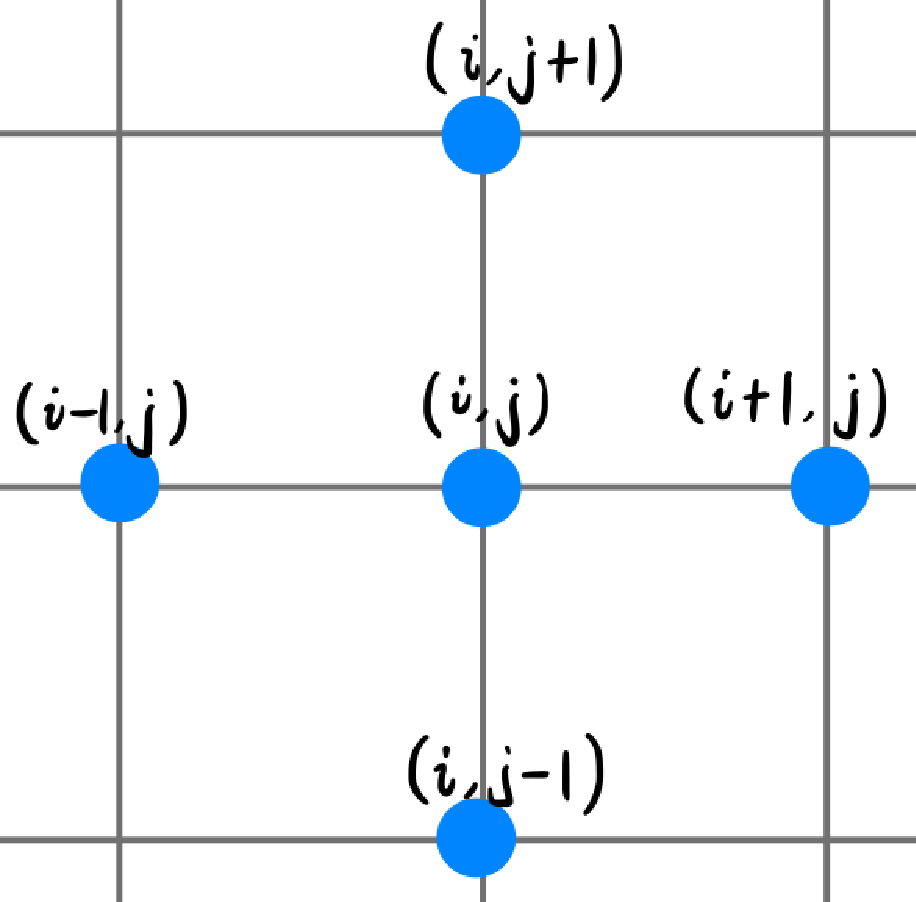
\includegraphics[width=.6\textwidth]{./figs/disc}
    \caption{\label{fig:disc} Finite centered difference on 2D.}
\end{figure}

For the relaxation method, we use this equation, start from the boundary, and iterate until we get the desired accuracy. Here we look at this equation in a different way. We should notice that the value at one point is the statistical average of its neighbours' values. So we can regard the $\frac{1}{4}$ as the statistical weight of each neighbour while calculating the value of the center point. Then we can construct the Monte Carlo method based on this point of view.

\subsection{Simple Random Walk Method}

\begin{figure}[htbp]
    \centering
    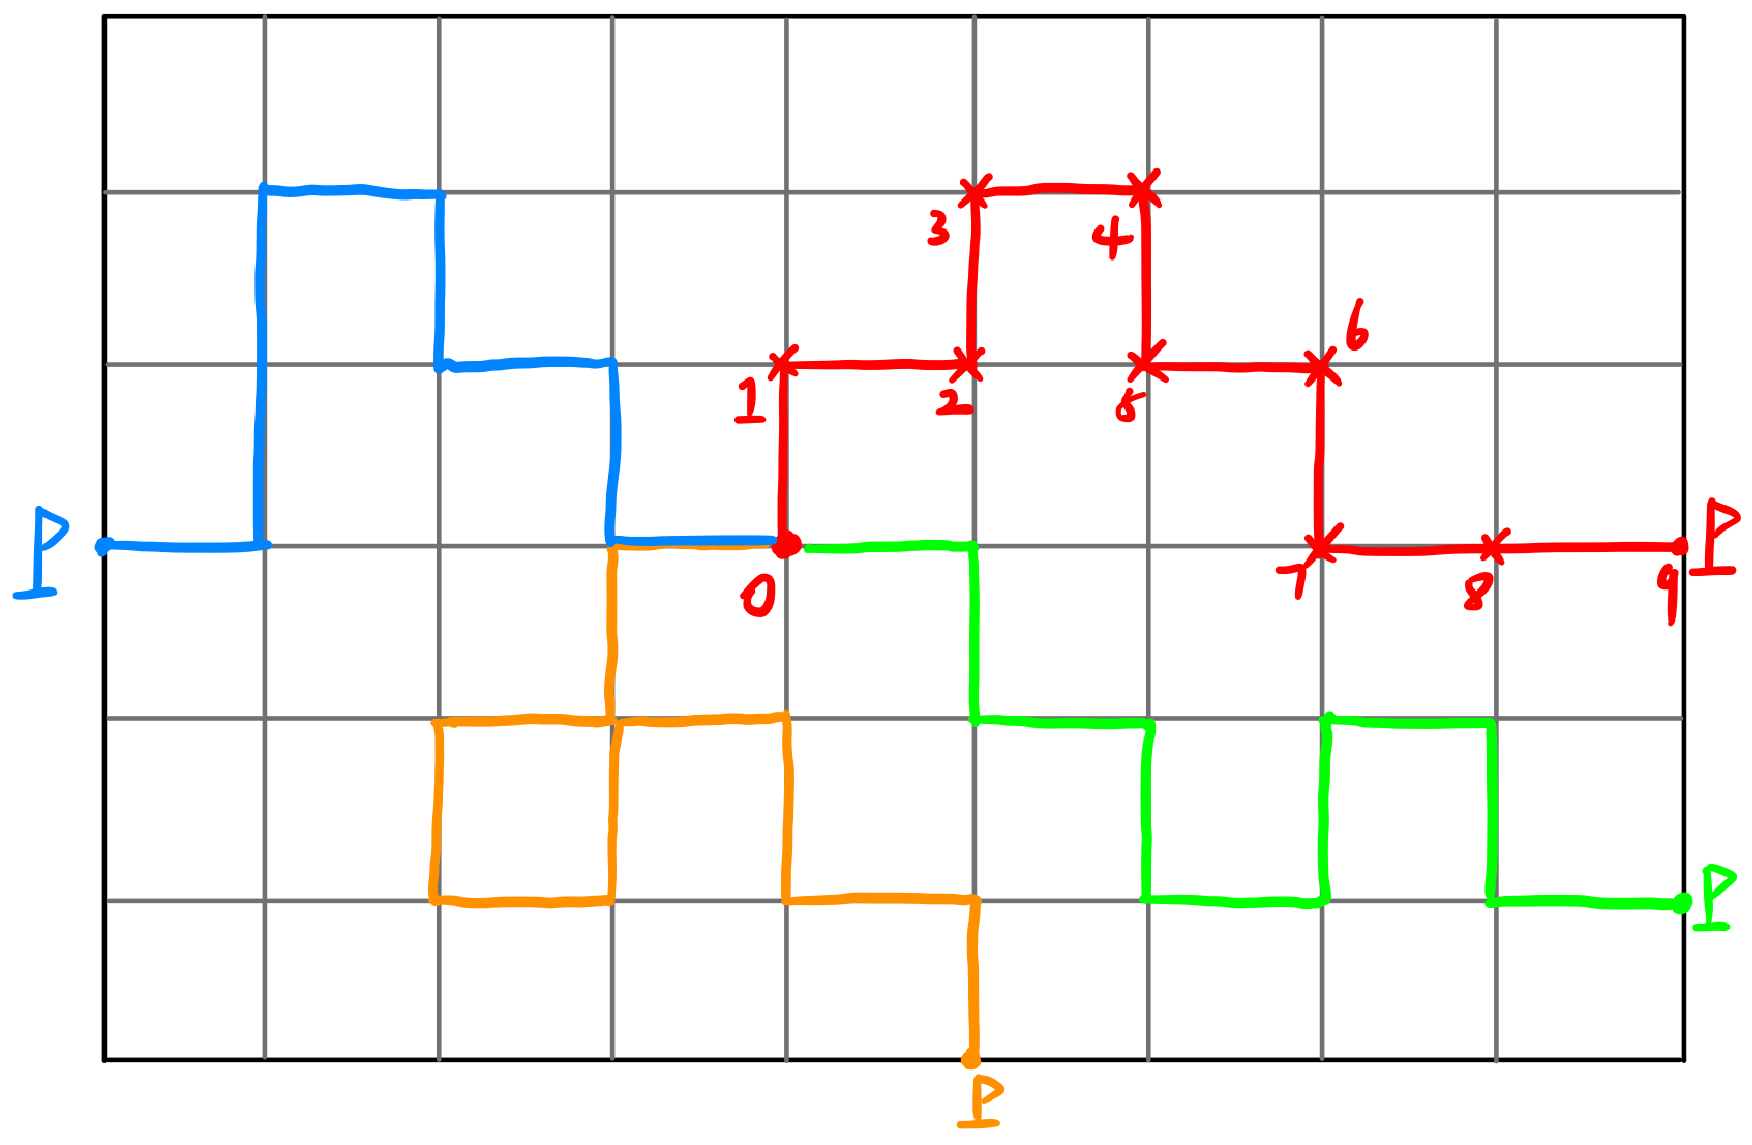
\includegraphics[width=.8\textwidth]{./figs/srw}
    \caption{\label{fig:srw} Simple Random Walk method.}
\end{figure}

Given the point $P_0$ whose value we want to evaluate on the grid,
\begin{enumerate}
    \item Pick a neighbour point randomly, e.g. $P_1$, with proper probability distribution, here it's $\frac{1}{4}$ for each point.
    \item We don't know the value at $P_1$, but we know it's the average of its neighbours, so pick one of it's neighbours randomly with proper probability distribution, e.g. $P_2$. Continue this process, until we reach a point on the boundary, e.g. $P_n$, whose value is given.
    \item We know that $P_n$ is an estimate of $P_{n-1}$, which is an estimate of $P_{n-2}$, etc, etc, all the way back to $P_0$. So after this random walk process, we get the value of $P_n$ as an estimate of $P_0$.
    \item As a typical Monte Carlo method, we do a large amount of random walks from $P_0$ to the boundary, then average all the estimates. We can get a good estimate of the value at $P_0$, whose accuracy depends on the number of random walks, i.e. the number of estimates.
\end{enumerate}
This is the process of the Simple Random Walk method, which is very straightforward based on the discrete form of the Laplace's Equation.

One more thing worth being mentioned here is that this method can be easily generalized for the Poisson's Equation,
\begin{equation}
    \nabla^2 u = q(x,y)
\end{equation}
with boundary value condition. The discrete form of Poisson's Equation reads,
\begin{equation}
    u_{i,j} = \frac{1}{4} \qty(u_{i+1,j}+u_{i-1,j}+u_{i,j+1}+u_{i,j-1}) - \frac{1}{4} q_{i,j}.
\end{equation}
Then after one random walk process with $n$ steps, the estimate is given by,
\begin{equation}
    u_n - \frac{1}{4}\sum_{k=0}^{n-1}q_k,
\end{equation}
where $u_n$ is the value on the boundary and $q_k$'s are the values on the path. More details can be found in references, in the following discussion, we still keep concentration on the Laplace's Equation.

\subsection{Walk on Spheres}

As we should notice, for the Laplace Equation, one estimate given by one random walk is just the value at the point on the boundary where the random walk ends. So the estimate doesn't really depend on the path of the random walk. If we let the grid spacing go to zero, which obviously will increase the accuracy of the estimate, then the random walk here becomes simple Brownian motion.

Consider a sphere centered at $\bm{r}$, for a simple Brownian motion starting from $\bm{r}$, the possibility for the motion to reach any point on the sphere is the same. So since the path doesn't matter here for the Laplace equation, why do we simulate the Brownian motion step by step? We can jump to one point on the sphere directly! This will lead us to the Walk on Spheres method.

\begin{figure}[htbp]
    \centering
    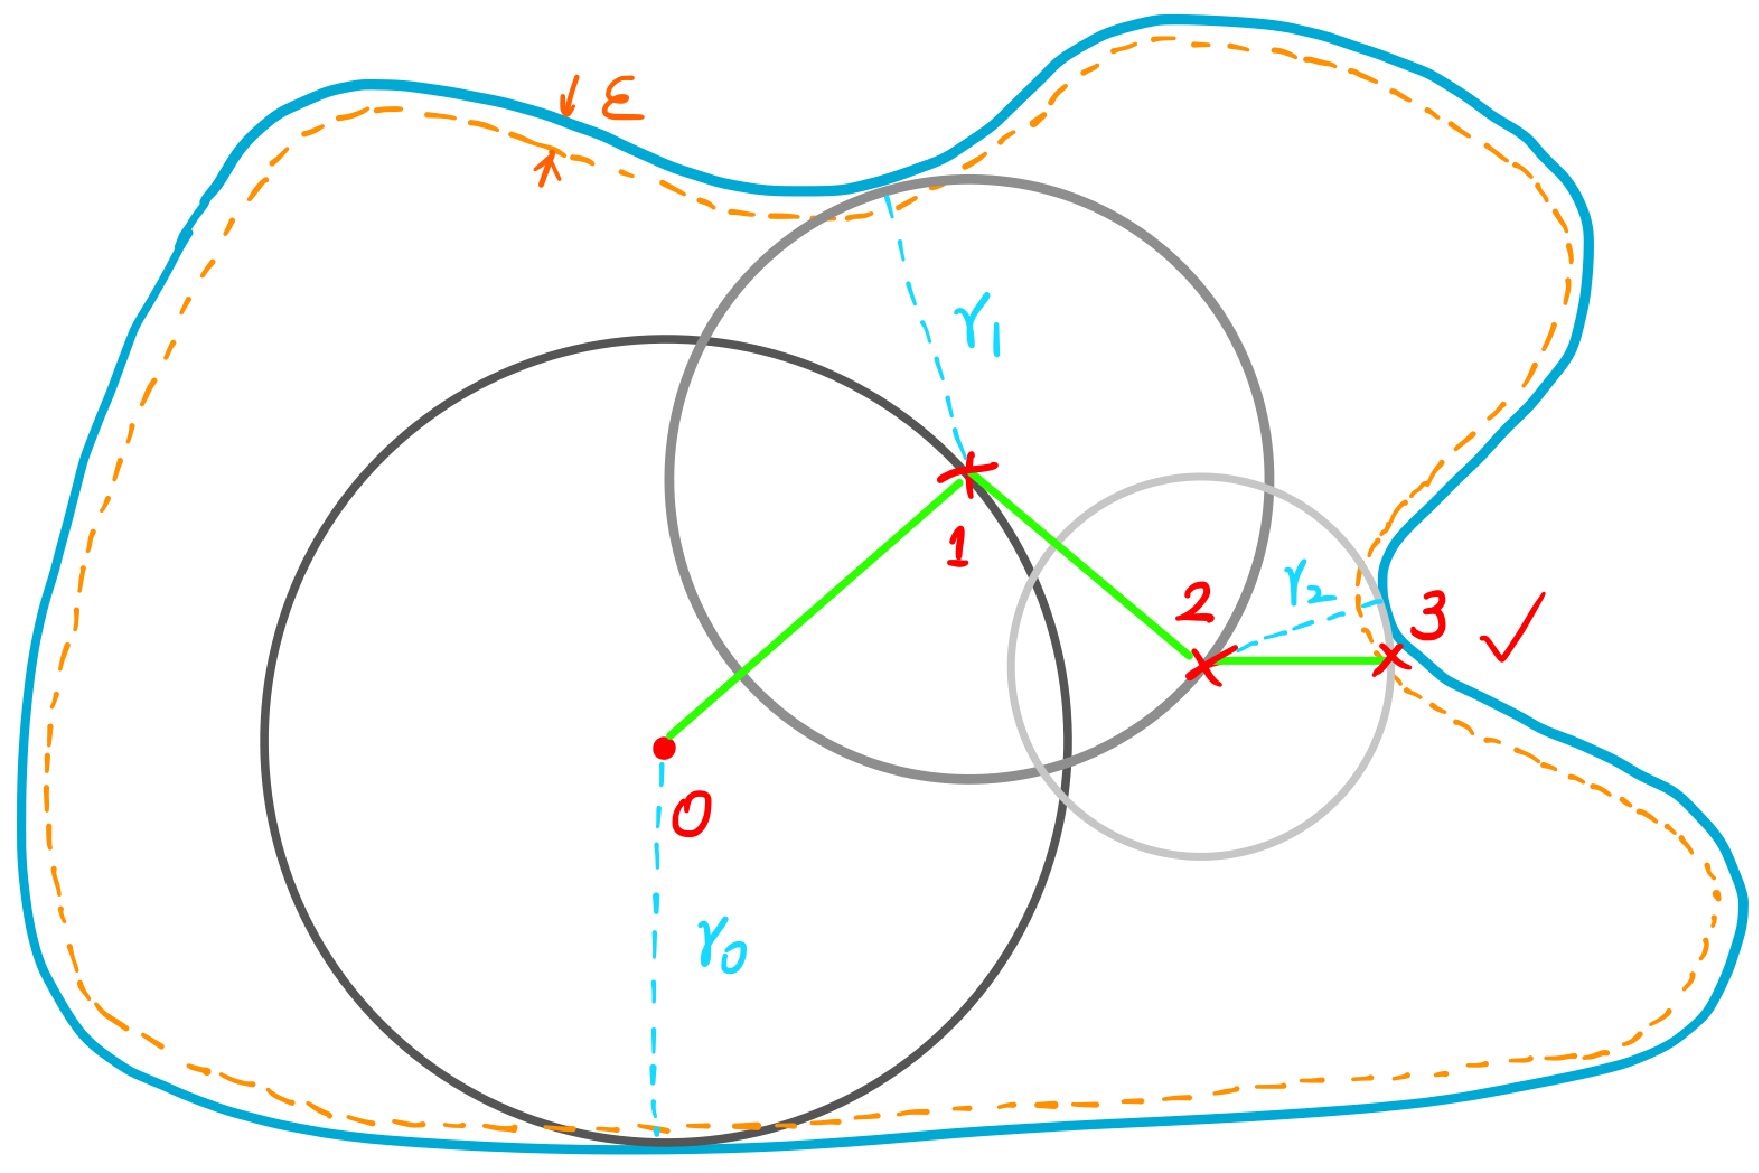
\includegraphics[width=.8\textwidth]{./figs/wos}
    \caption{\label{fig:wos} Walk on Spheres method.}
\end{figure}

The process of the Walk on Spheres (WoS) method is shown in FIG.~\ref{fig:wos}. Here are some explainations.
\begin{itemize}
    \item The radius of the spheres (circles in 2D) are determined by the shortest distance from the point to the boundary, e.g. $r_0$, $r_1$, and $r_2$ in FIG.~\ref{fig:wos}.
    \item The next point is chosen randomly on the sphere, e.g. points $1, 2, 3$ in FIG.~\ref{fig:wos}.
    \item Since the WoS method is grid-free, we use the shell with thickness $\epsilon$ to judge whether the random motion reaches the boundary, as shown in FIG.~\ref{fig:wos}.
\end{itemize}

Since most of the time in the Simple Random Walk method is wasted on the random walk, we can expect the WoS method to be much faster. Also, the WoS method is grid free, so there is no discretization errors. The error for one estimate is caused by the shell thickness $\epsilon$, which will be analyzed in the implementation section.

\subsection{Characteristics of Monte Carlo method}

Both the Simple Random Walk (SRW) and Walk on Spheres (WoS) methods are Monte Carlo methods. These Monte Carlo methods here have some characteristics and advantages that normal deterministic methods don't have.

\subsubsection{Independence of points}

The first thing to notice is that unlike the relaxation or Gauss-Seidel methods, the points on the grid for the SRW or on the grid-free WoS are totally independent. So it's very fast to estimate some point values instead of the whole space.

\subsubsection{Boundary \& Dimension}

For the Monte Carlo methods here, the boundary doesn't matter a lot. The only thing is to decide whether the random walk reaches the boundary, and at which point. So it's relatively easy for these methods to handle some problems with complex boundaries. Also, it's easier for these methods to be extended to higher dimensions.

\subsubsection{Parallel Computing}

Not only different points, as mentioned above, but also different estimates for one point are independent. So these Monte Carlo methods are naturally parallel. The two most straightforward ways to parallelize the program are,
\begin{itemize}
    \item Parallelize the different estimates for one point, then average the results from different processes.
    \item Parallelize the set of points to be evaluated.
\end{itemize}
In our simulation, we take the first way.

\section{Implementation \& Analysis}

In this section, we first introduce how the parallel programs are implemented. Then we use the methods to study two practical problems and analyze the properties of these methods.

\subsection{Parallelization in \emph{Python}}

In \emph{Python}, there are many packages for parallel computing. In this project, we use the \emph{multiprocessing} package. For a given set of points to be evaluated, we allocate the total number of independent estimates of every point to all available cores. Then we initialize the random number generators in all processes with different seeds. Here we use the \emph{numpy.random} module to produce random numbers, which can be initialized with \emph{numpy.random.RandomState(seed)}.

\subsection{Implementation on two boundary shapes}

\subsubsection{Square Boundary Problem}

\begin{figure}[htbp]
    \centering
    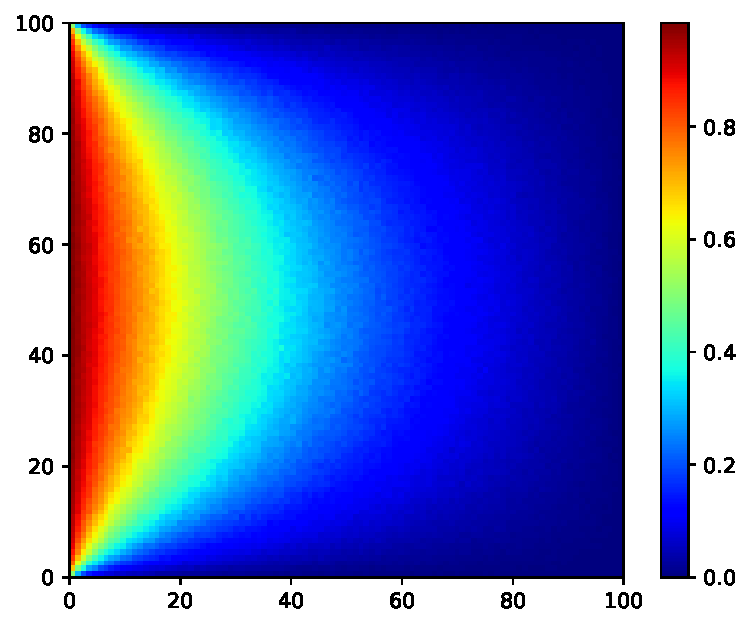
\includegraphics[width=.8\textwidth]{./figs/srw_s}
    \caption{\label{fig:srw_s} SRW method on 2D Square Boundary with Square Lattice, $100\times 100$ points, $5,000$ estimates for each point.}
\end{figure}

\begin{figure}[htbp]
    \centering
    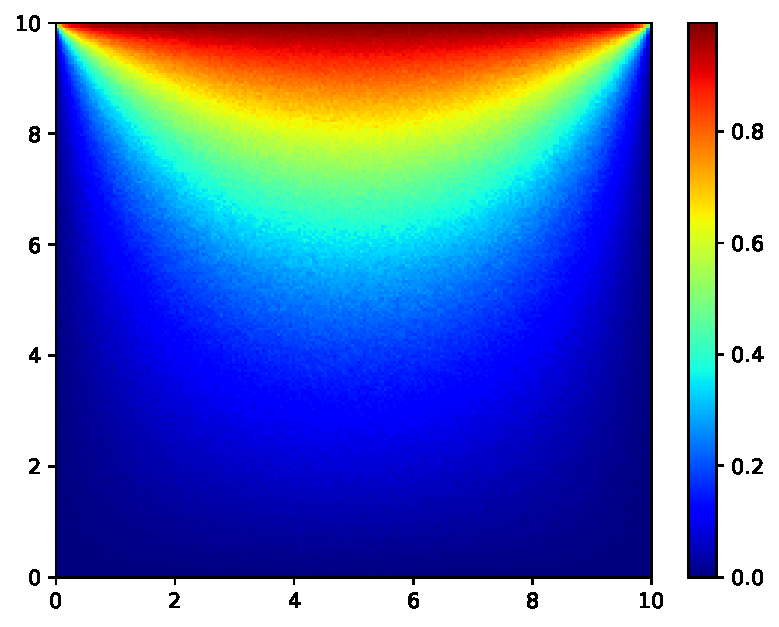
\includegraphics[width=.8\textwidth]{./figs/wos_s}
    \caption{\label{fig:wos_s} WoS method on 2D Square Boundary ($1,0,0,0$), $200\times 200$ points, $2,000$ estimates for each point.}
\end{figure}

Assume we have a 2D Laplace problem with the boundary given as a square. The results of the SRW method and the WoS method are shown in FIG.~\ref{fig:srw_s} and FIG.~\ref{fig:wos_s} seperately. For this problem, the SRW method took a few hours while the WoS method took only a few minutes. This shows that the WoS method is much faster than the SRW method, as we have expected.

\subsubsection{Circle Boundary Problem}

\begin{figure}[htbp]
    \centering
    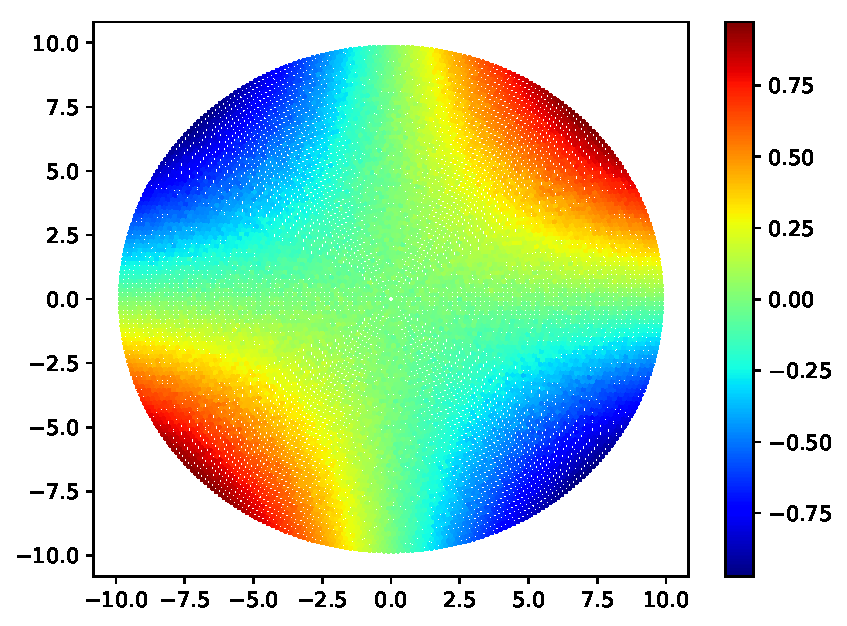
\includegraphics[width=.8\textwidth]{./figs/wos_c}
    \caption{\label{fig:wos_c} WoS method on 2D Circle Boundary ($\sin2\theta$), $10,620$ points, $1,000$ estimates for each point.}
\end{figure}

Here we study the 2D Laplace problem with a circle boundary. The result of the WoS method is shown in FIG.~\ref{fig:wos_c}.

In the following sections, we will analyze some properties of the WoS method based on these two boundaries.

\subsection{WoS method - The Influence of $\epsilon$}

\begin{figure}[htbp]
    \centering
    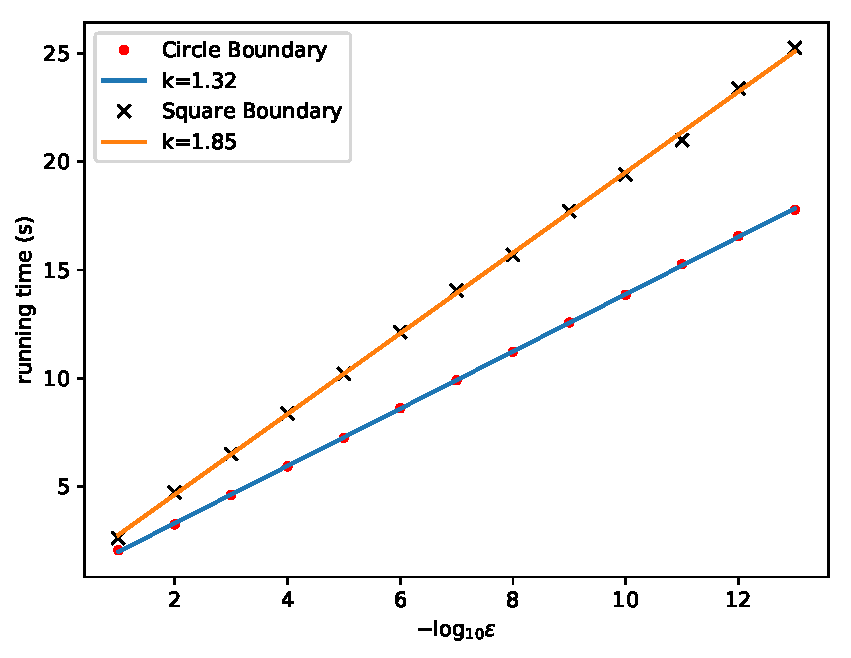
\includegraphics[width=.8\textwidth]{./figs/ep_t}
    \caption{\label{fig:ep_t} The running time - $\epsilon$ relation on both square and circle boundary.}
\end{figure}

For the Walk on Spheres method, here we study the influence of the shell thickness $\epsilon$ on the running time of the program. We evaluate a certain set of points with a fixed number of estimates for each point. The relation between the running time and $\epsilon$ is shown in FIG.~\ref{fig:ep_t}. As we can see, for the two boundaries we simulate here, the square boundary and the circle boundary, the relation between the running time $t$ and the shell thickness $\epsilon$ goes like,
\begin{equation}
    t = -k\log\epsilon + t_0,
\end{equation}
where $k$ and $t_0$ depend on the shape of the boundary and the set of points to be evaluated. This logarithmic relationship here means that we can decrease the order of magnitude of $\epsilon$ to increase the accuracy of the estimates with an acceptable cost of time.

\subsection{WoS method - Convergence}

\begin{figure}[htbp]
    \centering
    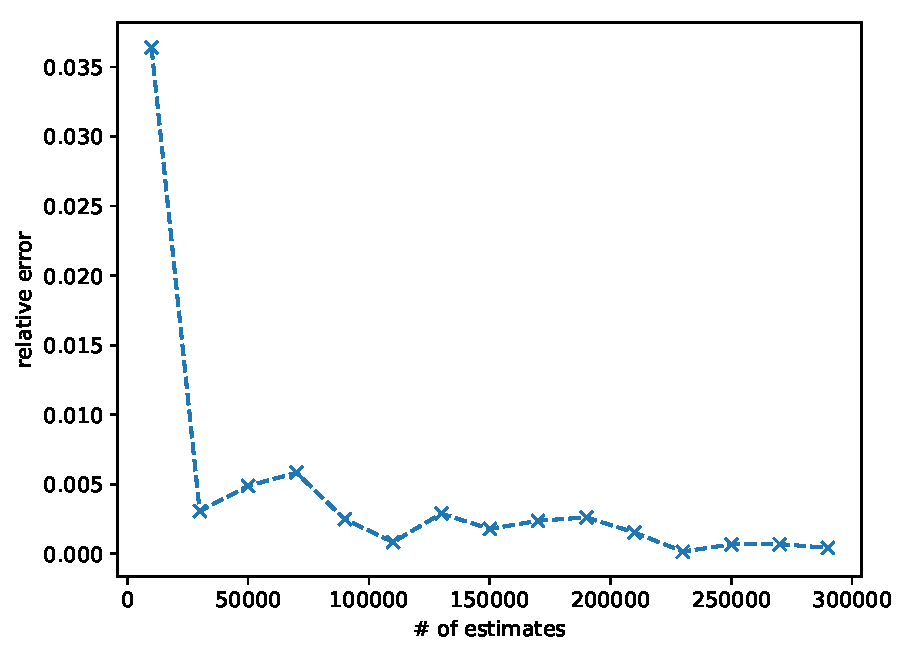
\includegraphics[width=.8\textwidth]{./figs/err_es}
    \caption{\label{fig:err_es} The convergence of the WoS method at the center point of the square boundary.}
\end{figure}

Here we study the convergence of the Walk on Spheres method. We pick the point at the center of the square bounadry, and study how its value changes with the number of estimates. The result is shown in FIG.~\ref{fig:err_es}. As we can see, the error decreases as the number of estimates increases, but we haven't found a proper scaling behavior.

\section{Future Work}

The time for this final project is limited, and there are still many things which are very interesting. Some future work directions include,
\begin{itemize}
    \item \emph{Green's Function First Passage}:
    \begin{equation*}
        p(x_0, x) = \pdv{G(x_0, x)}{n}
    \end{equation*}
    If we know the Green's Function for a domain, we can directly simulate the transition from the starting point to the boundary. Then we can get all the estimates directly.
    \item \emph{Parallelization on GPU}:\\
    The Monte Carlo methods here are naturally parallel, so they may be accelarated a lot with GPU computing.
    \item \emph{How things work for other PDEs}:\\
    e.g. Diffusion Equation etc.
\end{itemize}
Currently I am still trying to learn the GPU parallelization.

\section{Acknowledgement}

I'd like to thank Prof. Andrew MacFadyen for his instructive lectures during the class. I would also like to thank TA Marc Williamson for helpful discussions.

\section{References}

\begin{itemize}

    \item Gregory F. Lawler.
    \textit{Random Walk and the Heat Equation}
    \\\texttt{http://www.math.uchicago.edu/\~{}lawler/reu.pdf}

    \item Kevin Hu.
    \textit{Partial Differential Equations and Random Walks}
    \\\texttt{http://www.math.toronto.edu/courses/mat394h1/20139/Random\_Walk\_and\_PDE\_1.pdf}

    \item Eric Guan.
    \textit{Random Walks in $Z^d$ and the Dirichlet Problem}
    \\\texttt{http://www.math.uchicago.edu/\~{}may/VIGRE/VIGRE2011/REUPapers/Guan.pdf}

    \item
    \textit{Monte Carlo Methods in Partial Differential Equations}
    \\\texttt{http://www.hep.fsu.edu/\~{}berg/teach/mcmc05/homework/Fleming\_PDEs.ppt}

    \item Michael Mascagni.
    \textit{Monte Carlo Methods and Partial Differential Equations: Algorithms and Implications for High-Performance Computing}
    \\\texttt{https://engineering.jhu.edu/ams/wp-content/uploads/sites/44/2015/04/\\Exascale\_Mascagni.pdf}

    \item K.K.Sabelfeld and N.A.Simonov.
    \textit{Random Walks on Boundary for Solving PDEs}
    \\\texttt{http://citeseerx.ist.psu.edu/viewdoc/download?doi=10.1.1.12.7107\&rep=rep1\&type=pdf}
\end{itemize}

\end{document}
